\chapter{Methods}\label{chap:methods}
\todo{write methods introduction}
{\color{blue}
Chapter on tools (language models) used. What exactly do I want to explain?
First, a bit on how they work in general, second a bit of background on the models, a bit of a comparison (architecture and benchmarks?)
}

% background is more general, methods is specific to the methods we use, in our case LLMs

\section{Language Model Basics}\label{sec:basics}
This Section aims to provide an overview and fundamental understanding of the underlying concepts and terminology of the language models used in this work.
The models part of the benchmark are introduced in \secref{models}.
We will first establish the fundamentals of the transformer architecture in \subref{transformer} and take a look at the development to a \acrlong{LLM} in \subref{llm} before combining a number of common adaptions to visualize how a modern transformer architecture often looks like in \subref{modern}.


\subsection{The Transformer Architecture}\label{sub:transformer}
\begin{figure}[!htb]
    \begin{centering}
        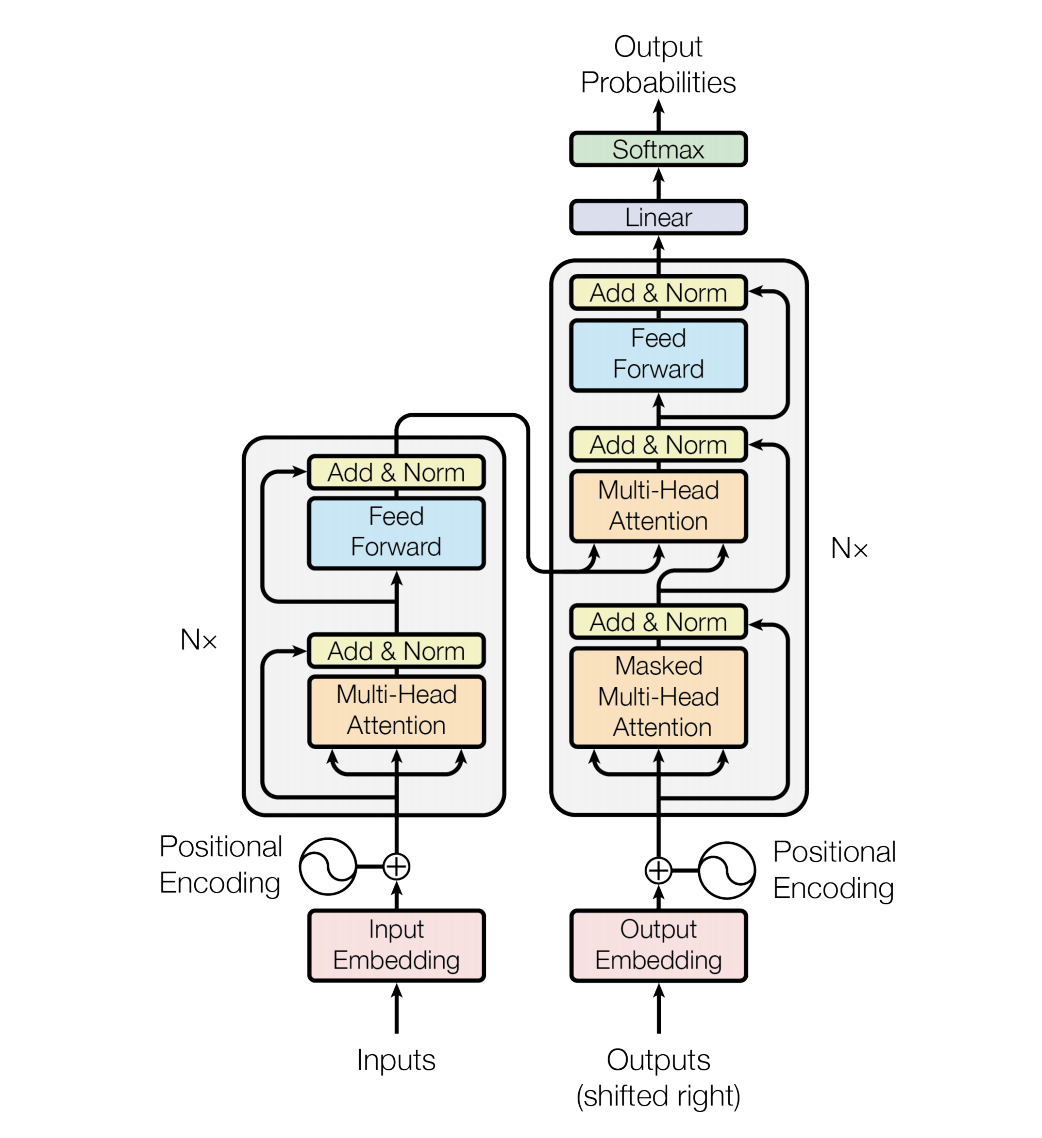
\includegraphics[height=0.5\textheight]{img/transformer}
        \caption[Original Transformer Architecture]{\textbf{Original Transformer Architecture.}
        The architecture was originally conceptualized for translation between languages.
        For that effect the text to translate (input) will be fully encoded to the embedding space, added to a positional encoding, and passed through alternating layers of self-attention and \gls{MLP} feed-forward layers with \gls{ReLU} activation, with residual connections and normalization after each.
        Output is generated autoregressively (generating each output token one-by-one, and append it to outputs to generate the next one), and has an additional layer of cross-attention to the input embedding.
        \Glspl{causal} are exclusively autoregressive decoder-only models.
        % The text to translate \textit{from} is the input, and the model will autoregressively (append selected output token to the outputs to generate the next output token until the full output has been generated) generate the full output.
        Image Source: \cite{vaswani_attention_2017}
        }
        \label{fig:transformer}
    \end{centering}
\end{figure}

% \begin{figure}[!htbp]
%     \begin{centering}
%         \subfloat[Runtime in minutes for correcting 25kb Matrix]
%         {\includegraphics[scale=0.9]{figures/results/runtime_25}} \\
%         % \caption[Correction time of 25kb]
%         % {\textbf{Runtime in minutes} for correcting the 25kb matrix.}
%         \subfloat[Runtime in minutes for correcting 50kb Matrix]
%         {\includegraphics[scale=0.9]{figures/results/runtime_50}}
%         \caption[Algorithm Runtimes]
%         {\textbf{Algorithm Runtimes} for correcting the different matrices. It
%         remains an open question why the difference between KR and RUST stays the
%         same, even though both ICE and RUST double their computation time. Smaller
%         is better.}
%         \label{fig:transformer}
%     \end{centering}
% \end{figure}


All modern language models are based on what Google introduced as the transformer architecture \cite{vaswani_attention_2017} in 2017, see the caption in \figref{transformer} for a more detailed description. \todo{actually include part on encoder and decoder in text here}
This new transformer architecture quickly established itself by outperforming other architectures available at the time with a fraction of the training cost.
An Encoder-Only transformer architecture, specifically \gls{BERT} set a new \gls{SOTA} for all \gls{NLP} benchmarks established at the time.

In 2019 \gls{OpenAI} introduced \gls{GPT2} \cite{radford_language_2019}, a very straightforward transformer architecture but scaled up more than previous models. \gls{GPT2} mainly demonstrated that bigger \glspl{LM} get more capable in general.
The biggest \gls{GPT2} variant had 1.5 billion parameters, which is 15x more parameters than the biggest \gls{BERT} variant had.
Others introduced models with similar parameter counts and capabilities.
\todo{figure out final main point I want to make}
% Along with significantly increasing capability in \acrlong{NLP}, these models enabled more sophisticated requests for data extraction.

% main difference to before: enabled more context compared to LSTM-based attention stuff (andscaling)

\subsection{Large Language Models}\label{sub:llm}
Models with more than a few billion parameters became generally referred to as a \acrlong{LLM}. \gls{GPT3}, the first such model with 176 billion parameters was introduced by \gls{OpenAI} in 2020 \cite{brown_language_2020}.
\glspl{LLM} differ from previous models in both parameter count (usually many billions) and substantial advances in general capability.
These models tend to have smaller siblings of the same architecture with fewer parameters, commonly in th steps of 7 billion, 13 billion, 30 billion, and 70 billion, though availability and exact parameter count varies.
Other Organisations trained \glspl{LLM} of this generation as well, some of them open-source, which demonstrated similar capabilities.
The most well-known models of this wave were \gls{BLOOM} and \gls{OPT} (throughout 2022).

The most recent and most capable generation of \glspl{LM} got introduced starting early 2023, after the release of \gls{ChatGPT} sparked worldwide interest in \glspl{LLM}. Progress happened fast and many incorporated numerous of the collectively found possible improvements. \glspl{LLM} of this generation are mostly classified so by their capability, and less so through parameter size, albeit their parameter counts still tend to be in the dozens of billions. Models of this category include the open-source \gls{llama} and its well-known derivatives \gls{alpaca} and \gls{vicuna}, \gls{falcon}, as well as most recently \gls{llama2}.

For more details on most of the aforementioned models, see \secref{models}.

\subsection{The Modern Transformer Architecture}\label{sub:modern}
See \figref{modern_transformer}.
\todo{rewrite subsection on modern transformer}

Over time, people figured stuff out. We have some explanations for why something works better, but most of it is still only speculation, and has been proven empirically more so than theoretically. 
One of the first things they found was that using SwiGLU as activation function instead of ReLU improved results. \todo{glossary / acronym entries for ReLU, SwiGLU, MLP?}
Instead of the previous sinusoidal positional encoding, they figured out that using \gls{RoPE} worked a lot better.
Also, normalization before, not after each sub-layer works a lot better.
As well as grouping some of the query heads for \gls{GQA}. This reduced parameters, speeds up evaluation and training, and delivers better results overall.
\begin{figure}[!htbp]
    \begin{centering}
        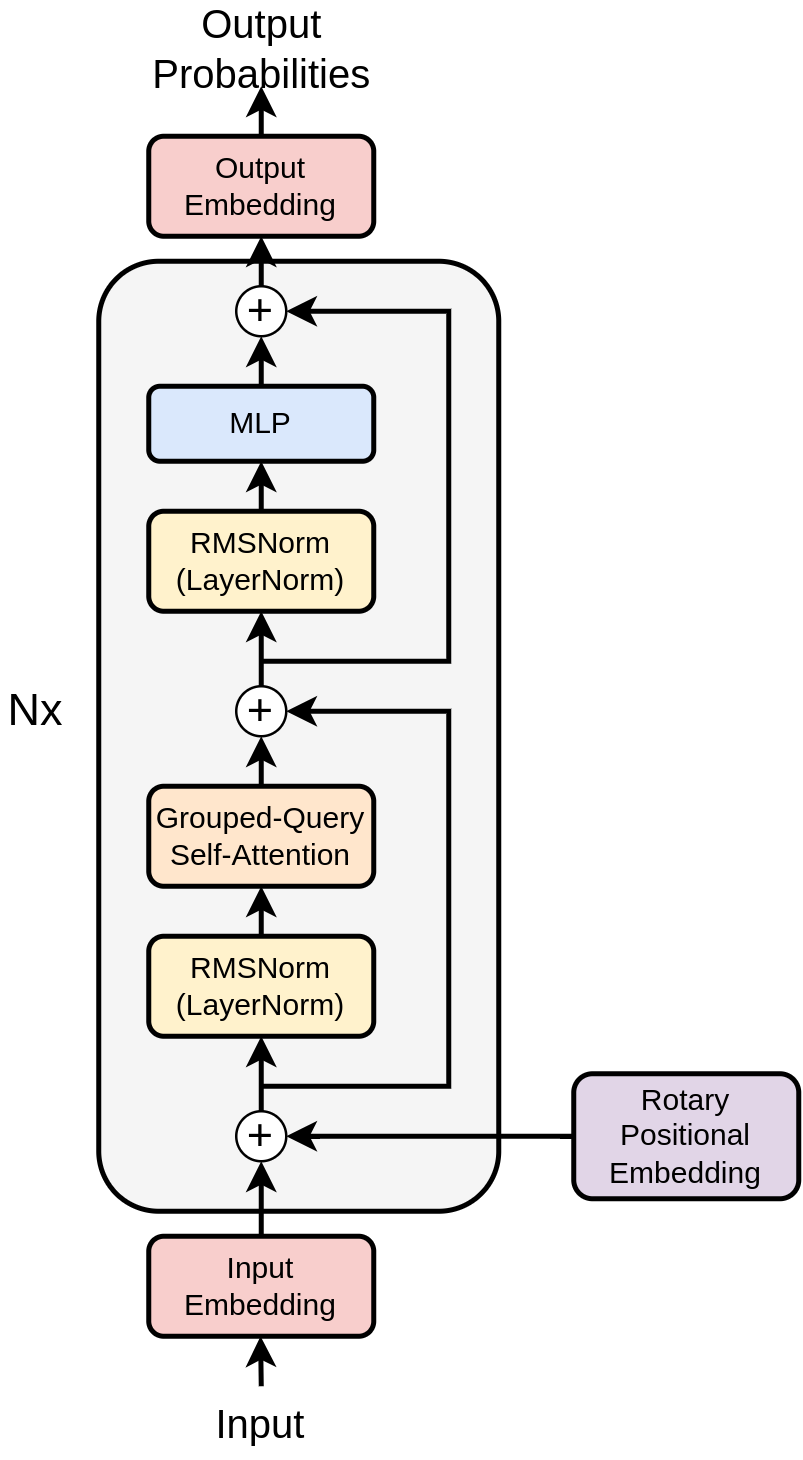
\includegraphics[height=0.8\textheight]{img/modern_transformer}
        \caption[Example of a Modern Transformer Architecture]{\textbf{Example of a Modern Transformer Architecture.} There are a number of differences when compared to the original architecture as seen previously in \figref{transformer}: layers are normalizing the residual with RMSNorm instead of having a normalized residual. Multi-head attention got replaced with \gls{GQA}, and sinusoidal positional embeddings with embeddings from \gls{RoPE} {\em on each layer}. Additionally, activation functions in the \gls{MLP} changed from \gls{ReLU} to \gls{SwiGLU}.}
        \label{fig:modern_transformer}
    \end{centering}
\end{figure}



\section{Training Methods}\label{sec:training}
\todo{write section on training methods}

\subsection{Pretraining}\label{sub:pretraining}
for main training usually crossentropy loss on text, decent batchsizes, large scale distributed.
\todo{write subsection on pretraining}

\subsection{Fine-Tuning}\label{sub:finetune}
specialized, mostly task-specific training making use of transfer-learning from a generalized model, making them capable for tasks where not much data is available
\todo{write subsection on finetuning}

\subsection{Fine-Tuning on Instructions}\label{sub:instruct}
mostly just changing 'expectation distribution' of model, giving preferred answers when interacting with the model for most people

a model fine-tuned on a instruction dataset or setting is commonly referred to as a 'instruct'-variant.
\todo{write subsection on instruction-finetuning}

\subsection{RLHF}\label{sub:rlhf}
learning preference policy to later fine-tune the large model on. basically lobotomization, as it drastically reduces capability.
\todo{this is not really relevant for my thesis. remove? or write?}

\section{Language Models Considered}\label{sec:models}
\todo{figure out basic parameters (e.g. release date) of models used}
\todo{list all models used, their sizes, and short background descriptions}
\todo{for each model, at the end, quickly put in one sentence why it was used / not used}
In this Section, we introduce the models used or considered for the benchmark.

See \secref{basics} for an overview and broad categorization of various models mentioned here.

\subsection{Criteria}\label{sub:criteria}
Setting out for our work, the only real constraint we had is that the model has to be any decently capable open-source \gls{causal}.

\subsection{OPT, BLOOM (Not Used)}\label{sub:opt}
\paragraph{OPT}\label{par:opt}
The initial model set out for this work was \gls{OPT} \cite{zhang_opt_2022}, a 175 billion parameter open-source \gls{LLM} trained by \gls{Meta}, with partially similar capability as \gls{GPT3}. During early literature research, we encountered the similar but slightly more capable \gls{BLOOM}.

\paragraph{BLOOM}\label{par:bloom}
\gls{BLOOM} \cite{workshop_bloom_2022} is a 176 billion parameter open-source \gls{LLM} trained by a cooperation of numerous organizations, spearheaded by \gls{hf} and \gls{Google}. When compared to \gls{OPT} across \gls{NLP} benchmarks, \gls{BLOOM} appears to perform marginally better.

\paragraph{Reasons for using neither}
The original plan for this work would use \gls{OPT} as only model. During early literature research, it seemed that \gls{BLOOM} would be slightly more capable, so we intended to try it with both, and compare them. 
While still in literature research, \gls{llama} got released, and with being seemingly both smaller and significantly more capable, as well as having properly scaled-down versions readily available, it was easy to make the call of going forward with \gls{llama} only. 
\todo{slightly rewrite to more academic writing style}
See \subref{llama} for more details on \gls{llama}.

\subsection{LLaMa (Used)}\label{sub:llama}
\gls{llama} is a suite of open-access \glspl{LLM} from \gls{Meta} with sizes ranging from 7 billion to 65 billion parameters, and capabilities comparable to, and sometimes beating \gls{SOTA} (including \gls{GPT3}) at the time \cite{touvron_llama_2023}. \gls{llama} can be seen as the culmination of distributed progress in one place.

\gls{llama} is not instruction fine-tuned. See \subref{instruct} for more details on instruction fine-tuning.
On instruction-finetuned variants of \gls{llama}, see \subref{alpaca} on Alpaca or \subref{vicuna} on Vicuna.

\subsection{Alpaca (Not Used)}\label{sub:alpaca}
The \gls{alpaca} Project \cite{tatsulab_2023} aims to build and share an instruction-finetuned \gls{llama} model.
Due to uncertainty with the \gls{llama} licence which this model is based on, no model weights where released officially.
They did, however, release everything else to easily fine-tune your own \gls{alpaca} when you already have the weights for \gls{llama}.
This becomes impractical for larger model variants due to increasing resource requirements. For this reason, we decided against including \gls{alpaca} in our benchmark.

See \subref{instruct} for more details on instruction fine-tuning.

\subsection{Vicuna (Used Partially)}\label{sub:vicuna}
\gls{vicuna} is a family of instruction fine-tuned \gls{llama}-variants, released by \gls{lmsys}. It is building on top of the training recipe of \gls{alpaca}.
However, not all weights of the corresponding \gls{llama} sizes are available.
The largest \gls{llama}-model (65B) does not have a corresponding \gls{vicuna} derivative available.

in chatbot arena: beating out \gls{llama} and \gls{alpaca} \cite{zheng_judging_2023}
\todo{write out in more detail}

See \subref{instruct} for more details on instruction fine-tuning.

\subsection{LLaMa 2 (Used)}\label{sub:llama2}
\gls{Meta} released \gls{llama2} a few months after \gls{llama}, in which they introduced few fundamental changes (making use of \gls{GQA} for the first time), trained on more tokens and released it under a different license. They also directly released its instruct variants.

See \subref{instruct} for more details on instruction fine-tuning.

\subsection{Falcon (Used)}\label{sub:falcon}
The \gls{falcon} \cite{zxhang_falcon_2023} family of language models are created by the Abu Dhabi-based \gls{tii}.
\gls{falcon} continues to dominate benchmarks with open-access models (in each respective parameter weight class), and also appears to rival some of the most capable closed-access models such as \gls{PaLM}.

Their better performance for most tasks is assumed to mostly the result of longer training and higher-quality data sets \cite{zxhang_falcon_2023}.

See \subref{instruct} for more details on instruction fine-tuning.

\subsection{GPT4 (Not Used)}\label{sub:gpt4}
\gls{GPT4} is the fourth generation \gls{GPT} model from \gls{OpenAI} \cite{openai_gpt4_2023}.
It is the single most capable \acrlong{LM} we currently know of.
However, it is not open-source and only accessible through an API provided by \gls{OpenAI}.
Additionally, \gls{OpenAI} continues to work on, change, and measurably degrade the capabalities \cite{chen_how_2023} of \gls{GPT4}, which makes it a bad target for comparison.
Even timestamped, supposedly 'unchanging' models have been observed to consistently change in behaviour \cite{jw1224_hn}.

\subsection{Final List}\label{sub:list}
In conclusion, we used the following models and sizes of the aforementioned:
\begin{itemize}
    \item \gls{llama} 7B, 13B, 30B, 65B (See \subref{llama} for more details on the model)
    \item \gls{vicuna} 7B, 13B (See \subref{vicuna} for more details on the model)
    \item \gls{llama2} 7B, 13B, 70B (See \subref{llama2} for more details on the model)
    \item \gls{falcon} 7B, 40B (See \subref{falcon} for more details on the model)
    \item \gls{falcon} (instruct variant) 7B, 40B (See \subref{falcon} for more details on the model)
\end{itemize}


% \begin{itemize}
%     \item Attention before transformers \url{https://jalammar.github.io/visualizing-neural-machine-translation-mechanics-of-seq2seq-models-with-attention/}
%     \item Let's build GPT: from scratch, in code, spelled out. \url{https://www.youtube.com/watch?v=kCc8FmEb1nY} from Andrej Karpathy
%     \item Alternative generative models: Denoising Diffusion probabilistic models
% \end{itemize}
